\documentclass[11pt]{article}
\usepackage[margin=1in]{geometry}
\usepackage{booktabs}
\usepackage{graphicx}
\usepackage{float}
\begin{document}
\section*{Supplementary Step 7 Visualization Report}
\subsection*{Overview}
\begin{tabular}{p{0.36\linewidth}p{0.54\linewidth}}
\toprule
Metric & Value\\
\midrule
Representative geometry session & PID001 / 2025-11-06\_008\\
Included participant-sessions from Step 7 & 36\\
Included questions in Step 7 trial table & 30\\
Abstract onset-locked epochs used & 539\\
Concrete onset-locked epochs used & 536\\
Epoch window & -3.5 s to 13.2 s around question onset\\
Baseline & -2.0 s to 0.0 s\\
Long-channel montage used in descriptive plots & 22 pairs (44 chromophore channels)\\
Primary Step 7 duration-aware p-value & 0.102262\\
\bottomrule
\end{tabular}
\paragraph{Adaptation note.} This report mirrors the Step~6 visualization bundle but anchors it to the Step~7 duration-aware cohort and primary model results. Because the Step~7 inferential model summarizes continuous fNIRS over variable-length windows, the descriptive topographic plots here remain onset-locked so that all trials share a common time base for direct visual comparison.
\paragraph{Rendering note.} As in the previous supplementary visualization reports, the sensor-geometry figure uses the participant digitization point cloud plus source, detector, channel, and pair geometry rather than an fsaverage brain-surface rendering, because the local \texttt{pyvista}/\texttt{fsaverage} stack is not available in this environment.
\subsection*{Step 7 Main Figures Reused}
\begin{figure}[H]
\centering
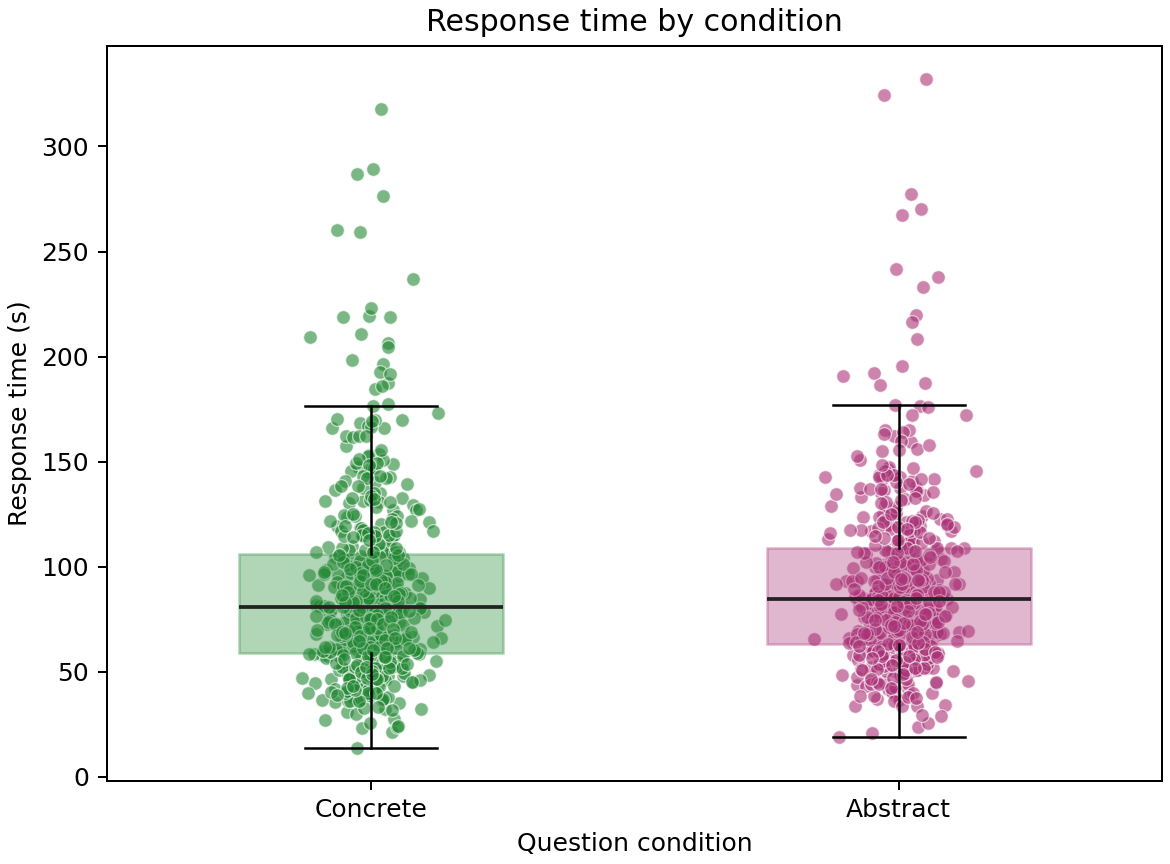
\includegraphics[width=0.48\linewidth]{../../figures/step7/response_time_by_condition.png}
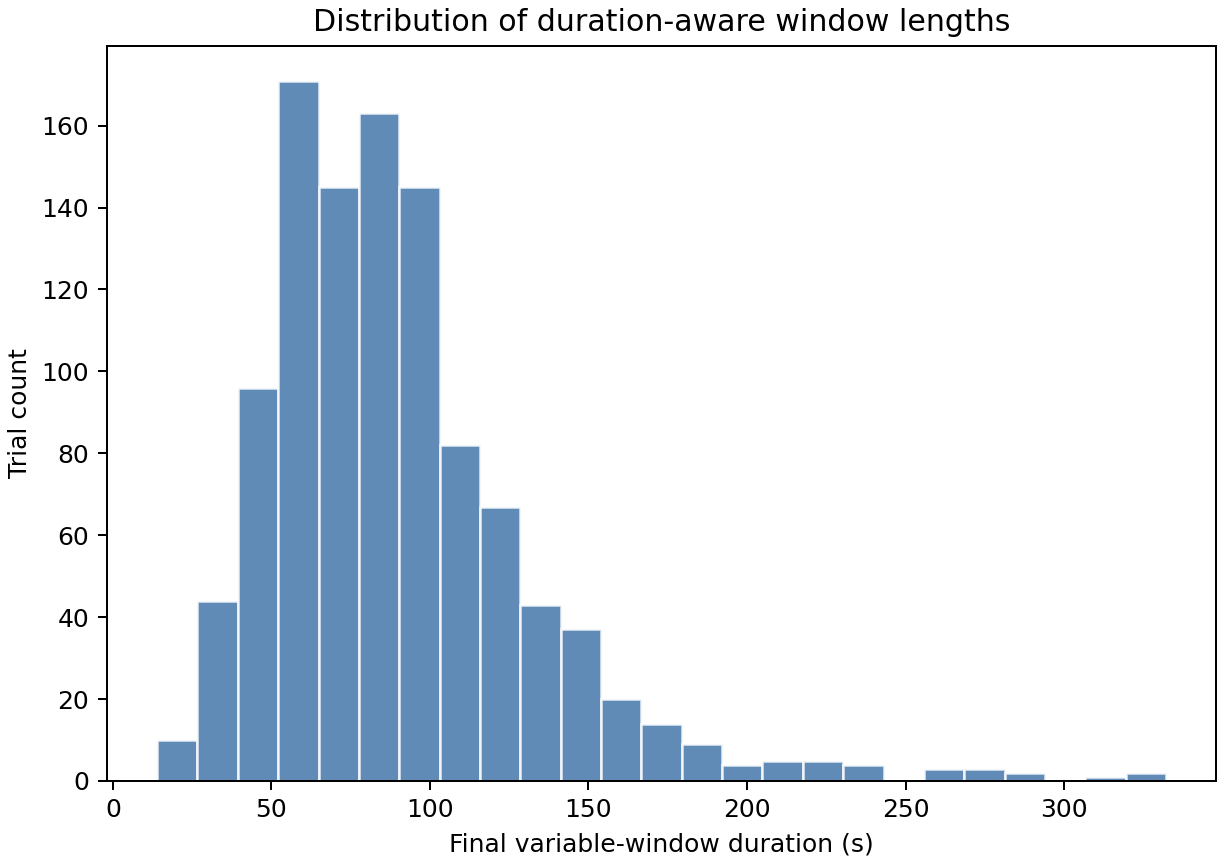
\includegraphics[width=0.48\linewidth]{../../figures/step7/variable_window_duration_histogram.png}
\caption{Step~7 duration diagnostics for response time by condition and the distribution of final variable-window durations.}
\end{figure}
\begin{figure}[H]
\centering
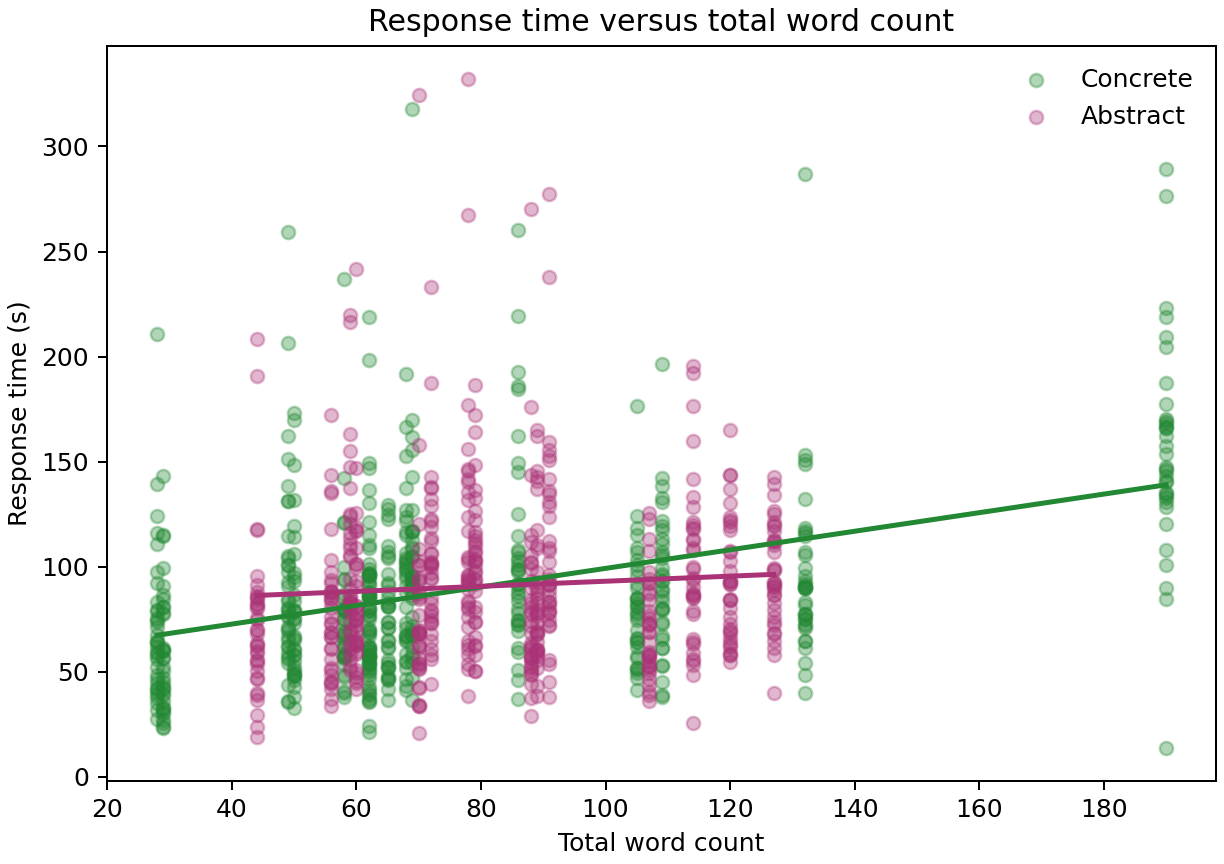
\includegraphics[width=0.48\linewidth]{../../figures/step7/response_time_vs_wordcount.png}
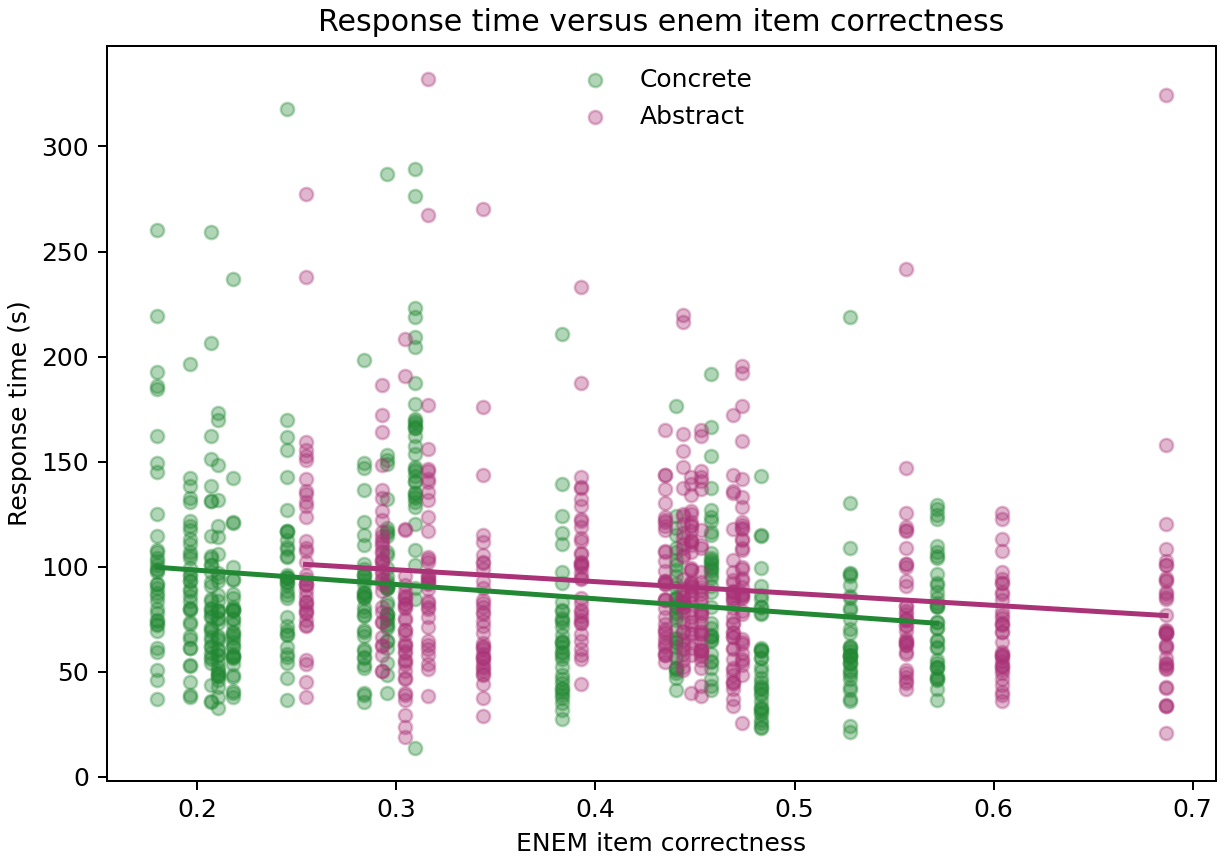
\includegraphics[width=0.48\linewidth]{../../figures/step7/response_time_vs_correctness.png}
\caption{Step~7 response-time associations with item length and ENEM item correctness.}
\end{figure}
\begin{figure}[H]
\centering
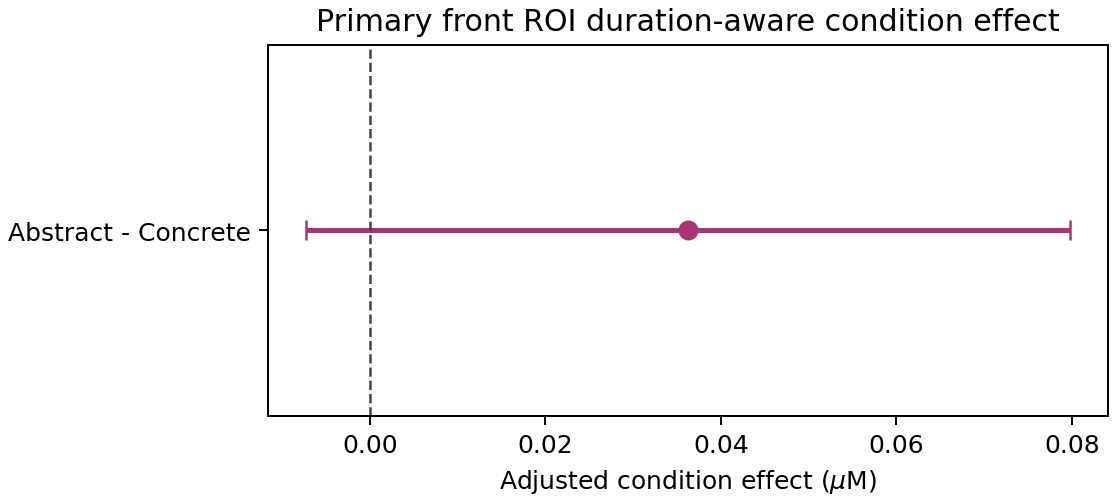
\includegraphics[width=0.48\linewidth]{../../figures/step7/front_roi_partial_effect_variable_window.png}
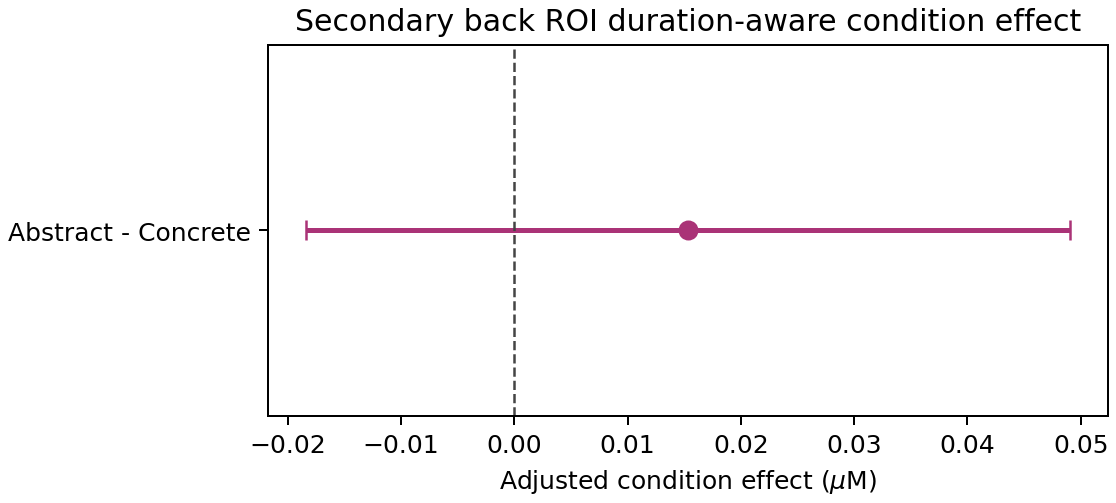
\includegraphics[width=0.48\linewidth]{../../figures/step7/back_roi_partial_effect_variable_window.png}
\caption{Step~7 duration-aware condition-effect summaries for the front and back ROI models.}
\end{figure}
\begin{figure}[H]
\centering
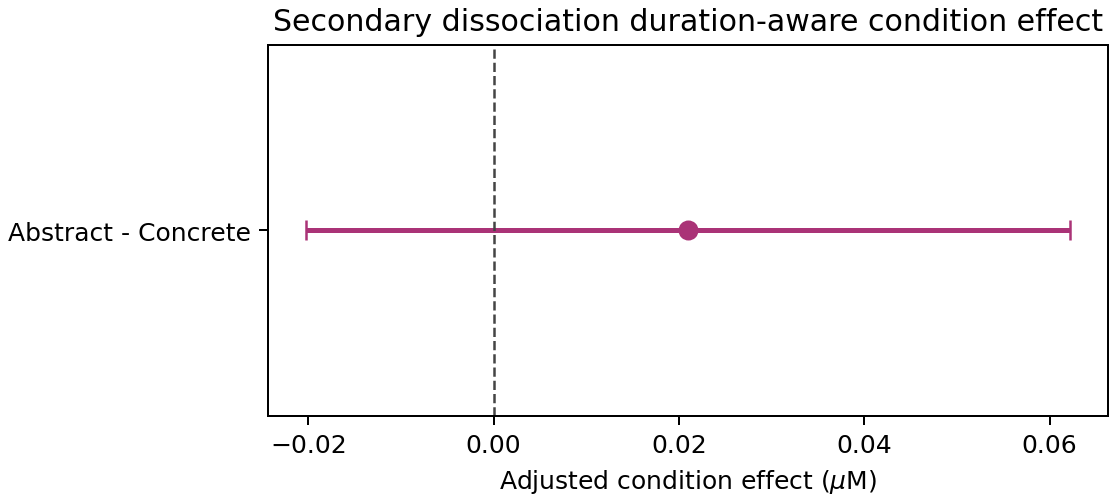
\includegraphics[width=0.48\linewidth]{../../figures/step7/dissociation_partial_effect_variable_window.png}
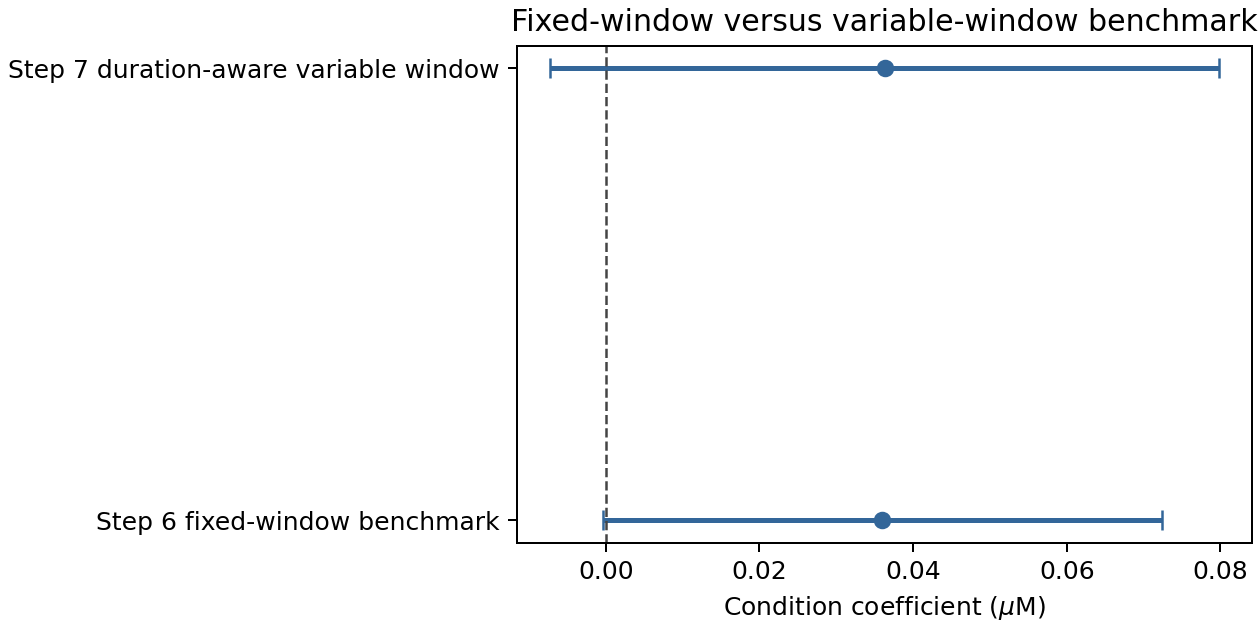
\includegraphics[width=0.48\linewidth]{../../figures/step7/fixed_vs_variable_comparison.png}
\caption{Step~7 dissociation effect and the direct benchmark against the Step~6 fixed-window model.}
\end{figure}
\begin{figure}[H]
\centering
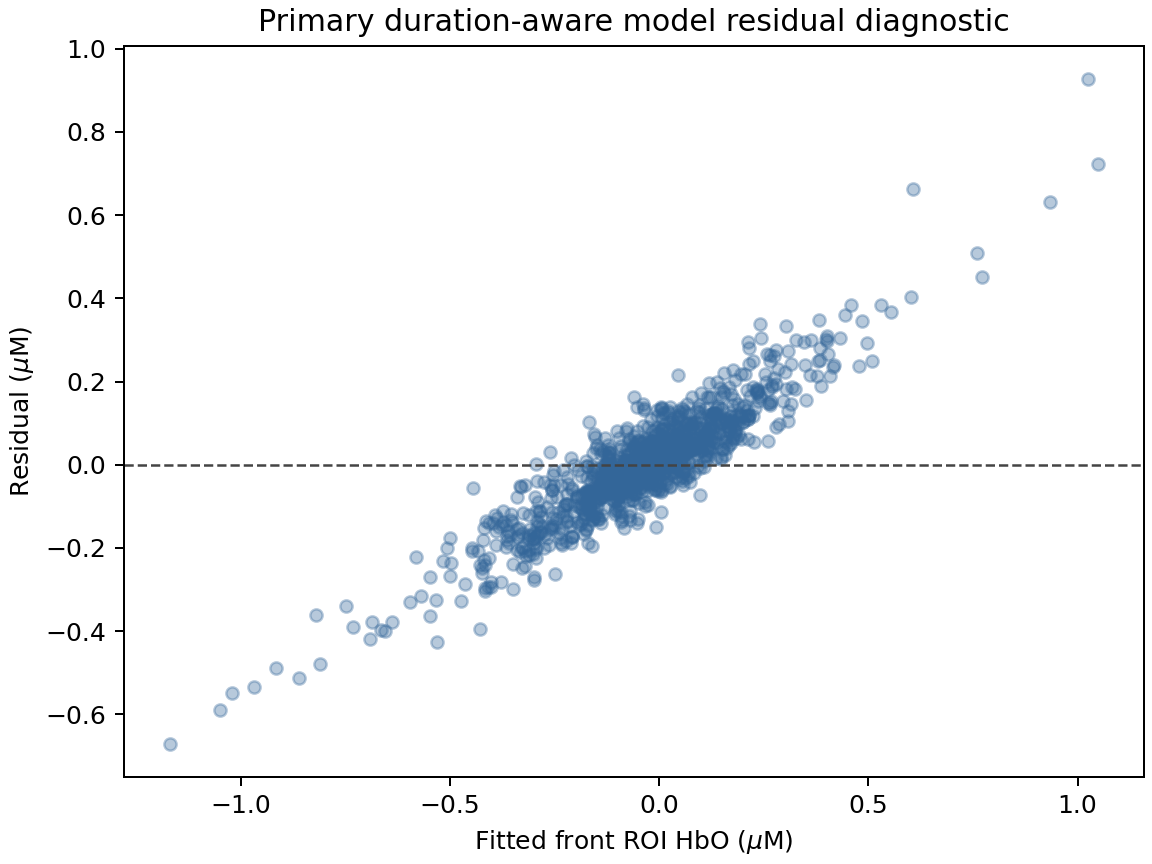
\includegraphics[width=0.72\linewidth]{../../figures/step7/model_residuals_primary.png}
\caption{Residual diagnostic from the Step~7 primary duration-aware model.}
\end{figure}
\subsection*{Step 6-Style Supplementary Plots for Step 7}
\begin{figure}[H]
\centering
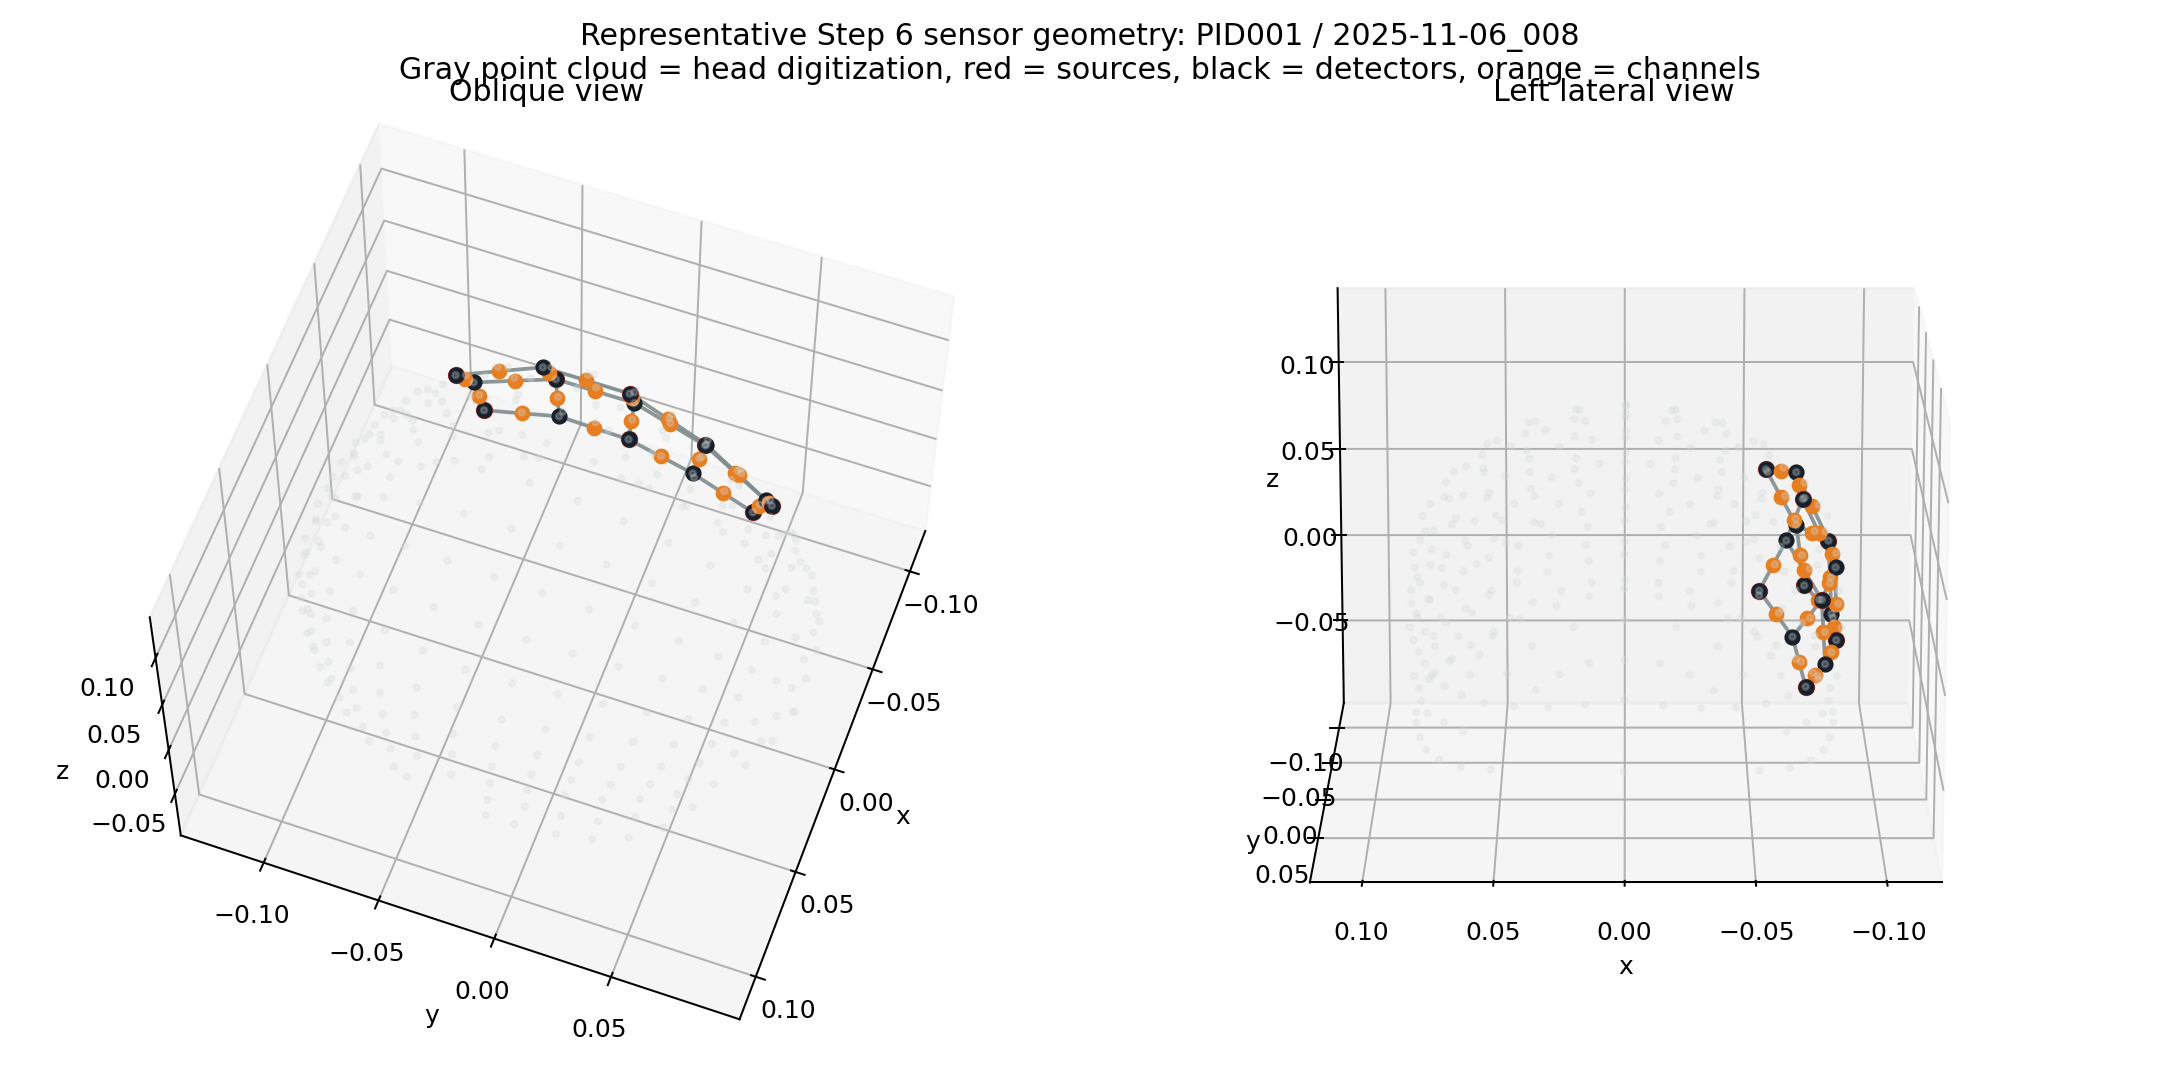
\includegraphics[width=0.95\linewidth]{../../figures/step7_visualization/representative_sensor_geometry.png}
\caption{Representative optode, channel, and source-detector-pair geometry for one Step~7 included participant-session. Short pairs are shown with dashed orange lines.}
\end{figure}
\begin{figure}[H]
\centering
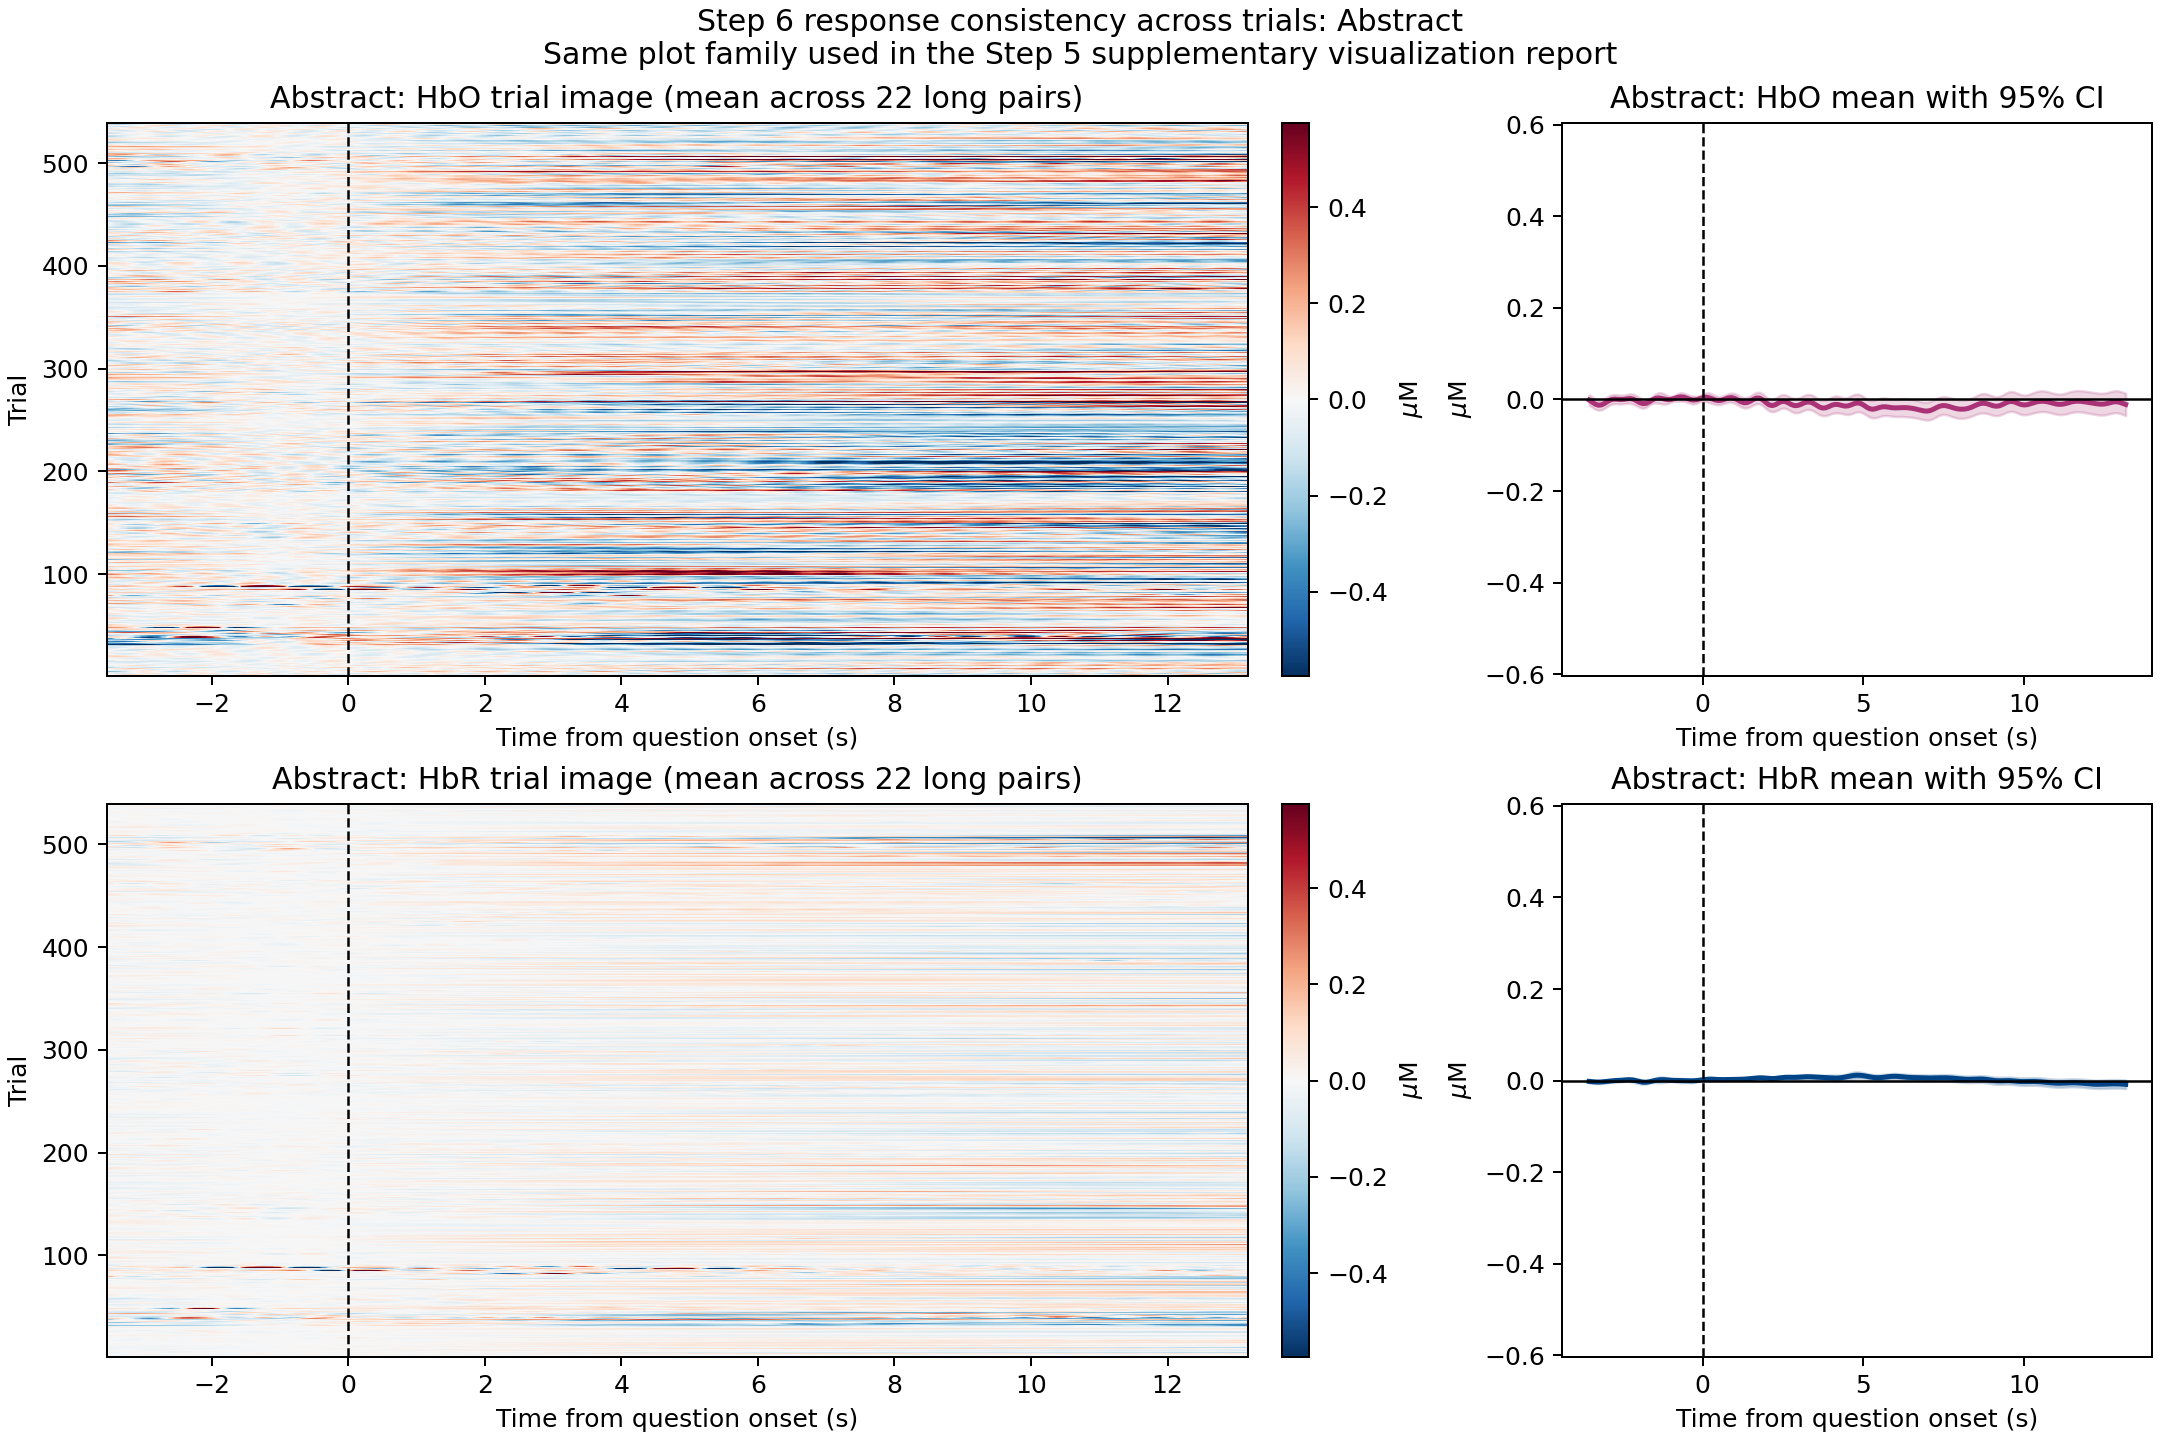
\includegraphics[width=0.48\linewidth]{../../figures/step7_visualization/abstract_trial_consistency.png}
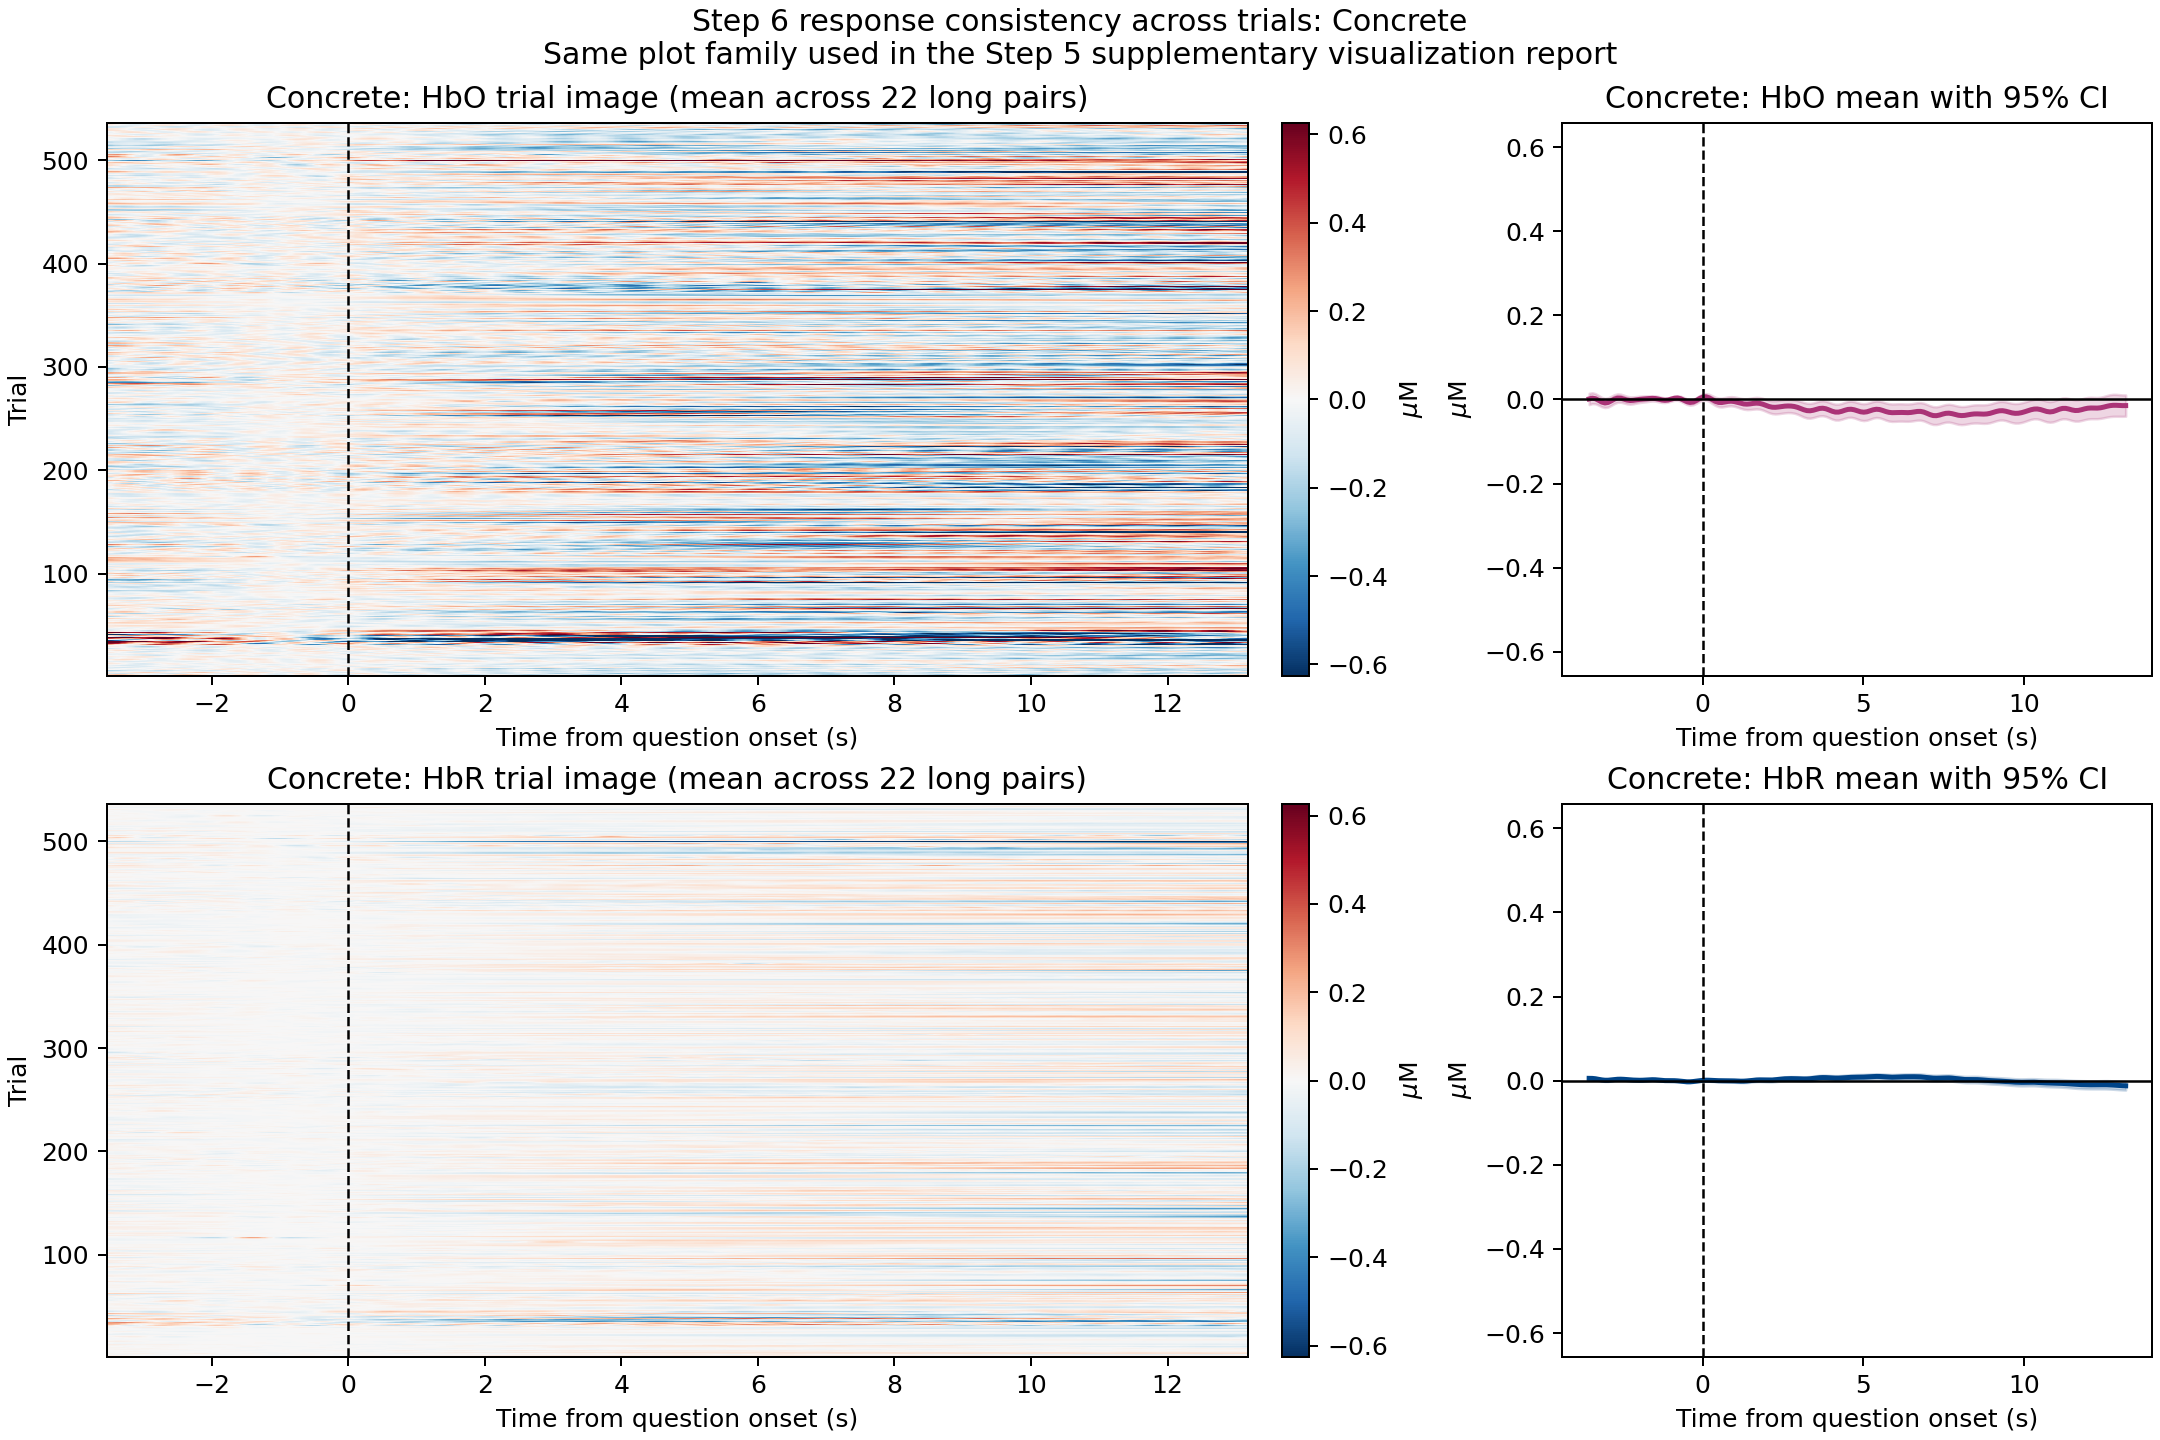
\includegraphics[width=0.48\linewidth]{../../figures/step7_visualization/concrete_trial_consistency.png}
\caption{Condition-adapted trial-consistency image plots for the Step~7 included trial set.}
\end{figure}
\begin{figure}[H]
\centering
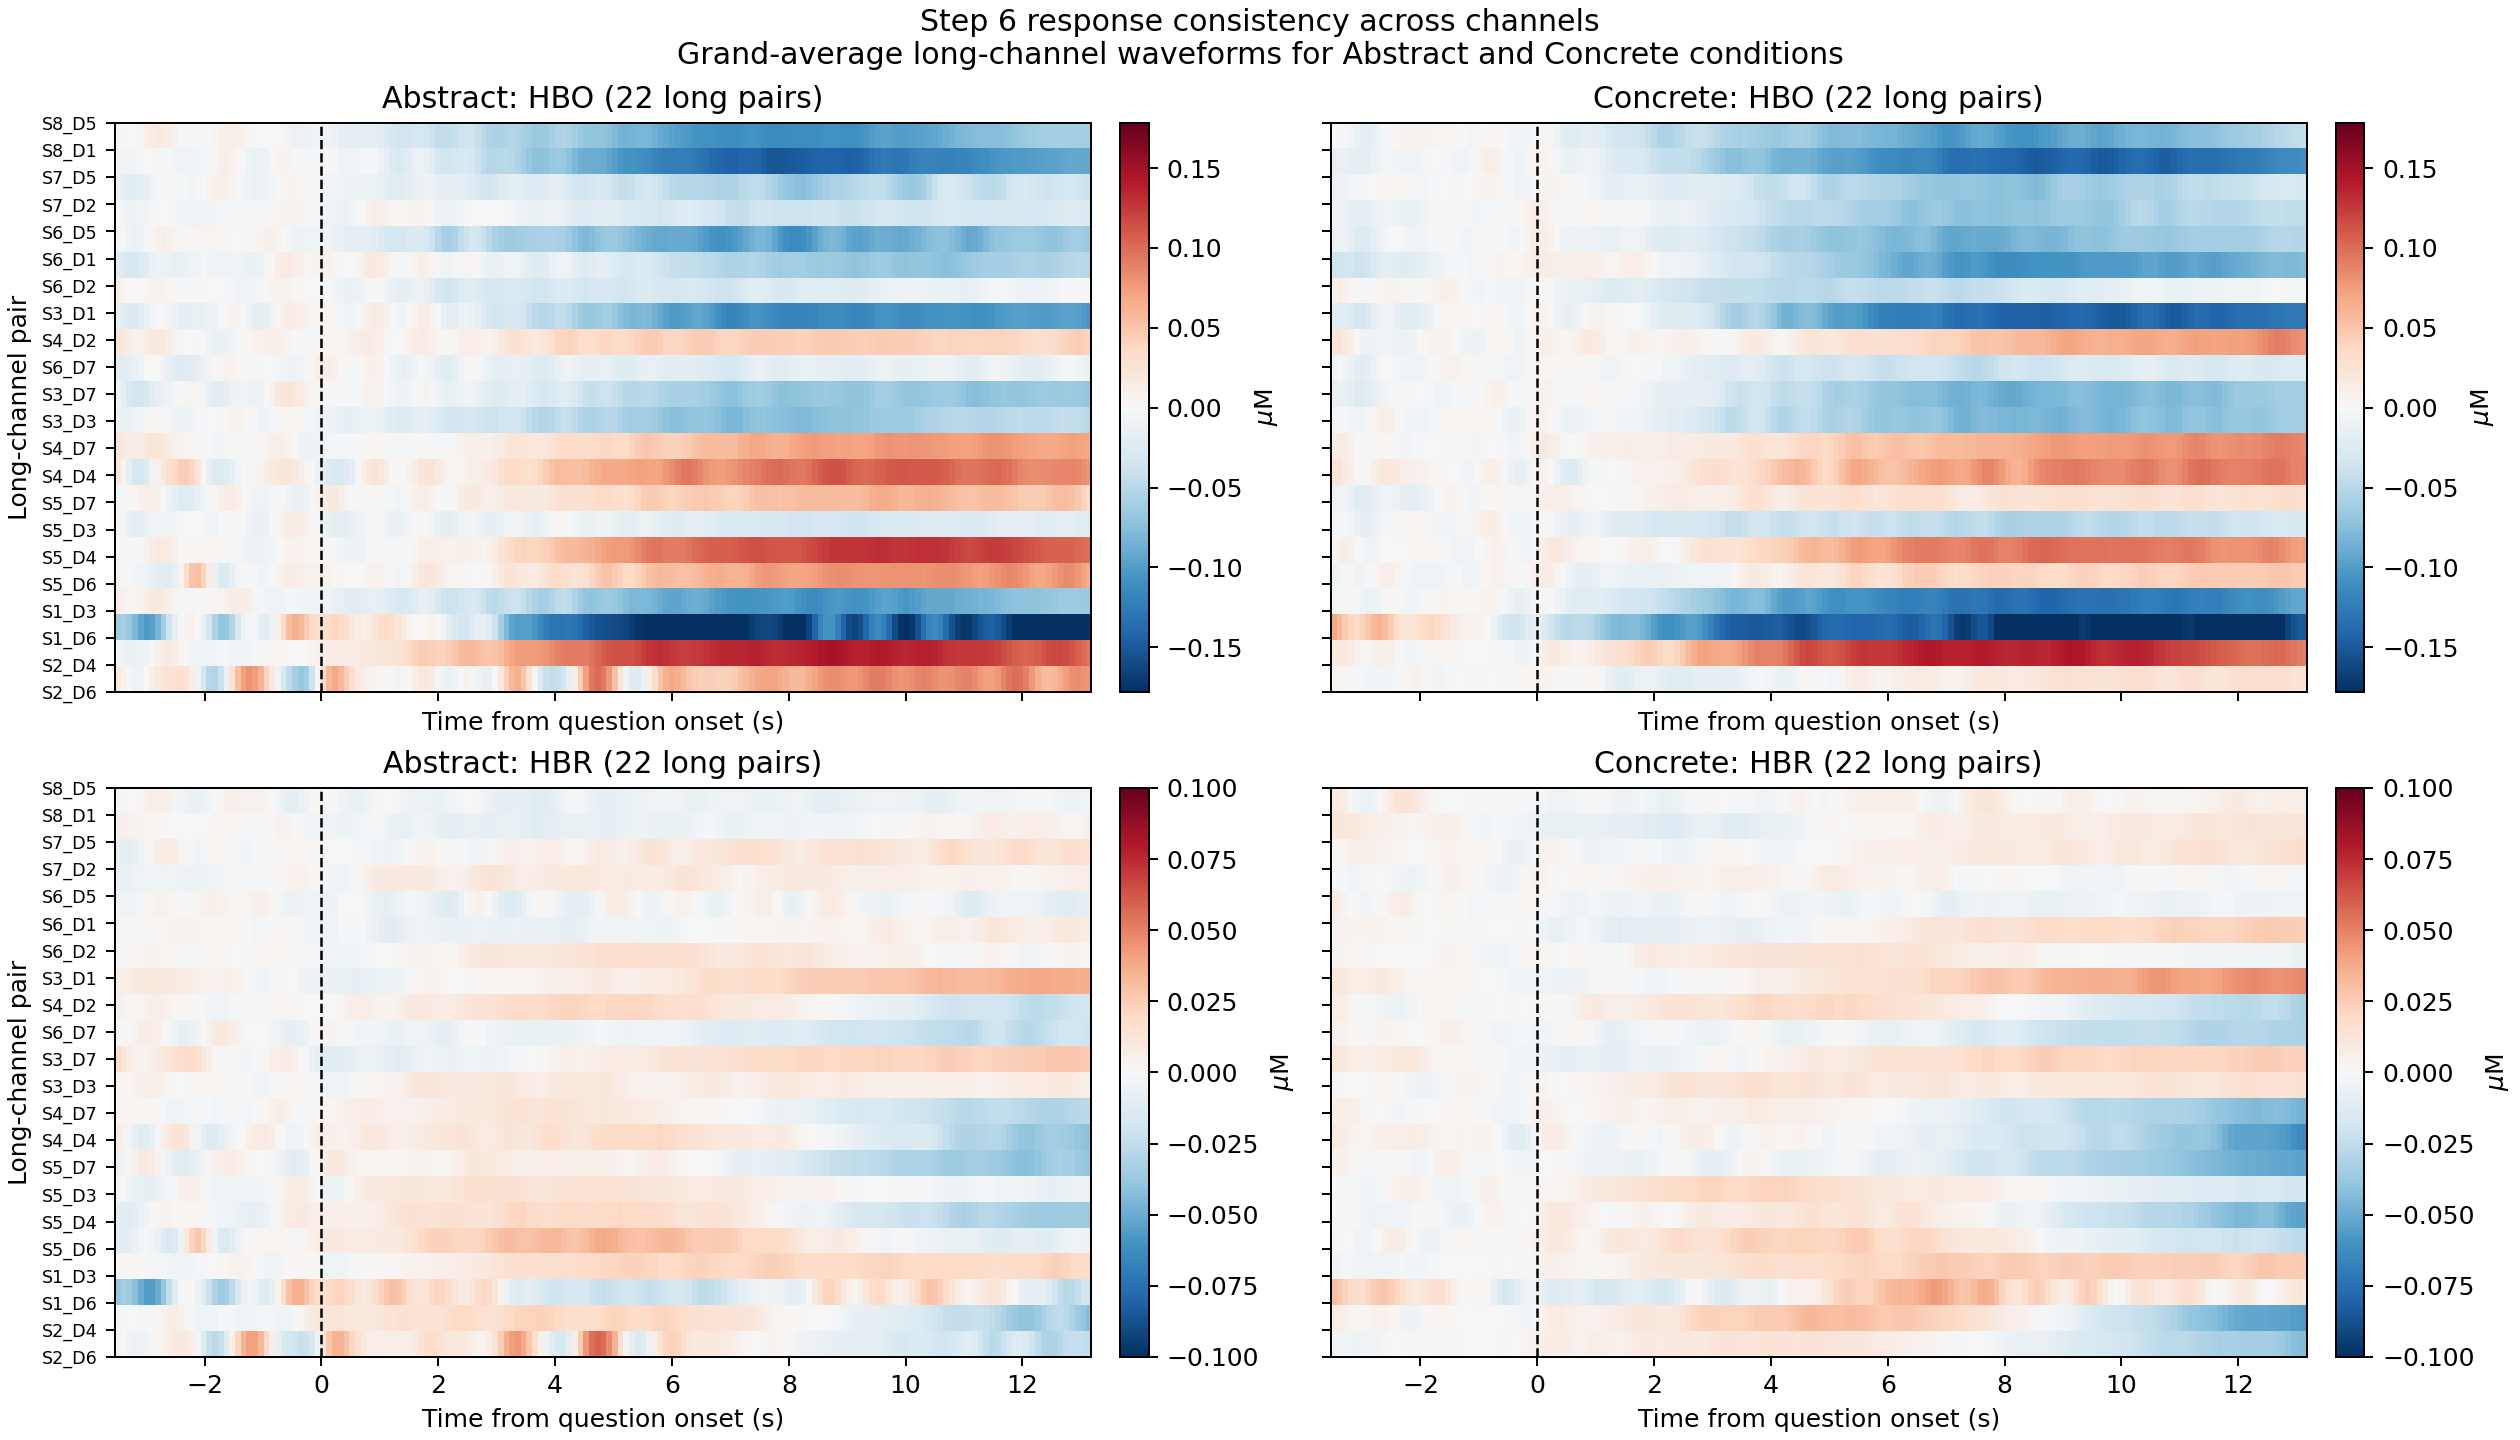
\includegraphics[width=0.95\linewidth]{../../figures/step7_visualization/channel_consistency_grid.png}
\caption{Grand-average long-channel response images across channels for the Abstract and Concrete conditions.}
\end{figure}
\begin{figure}[H]
\centering
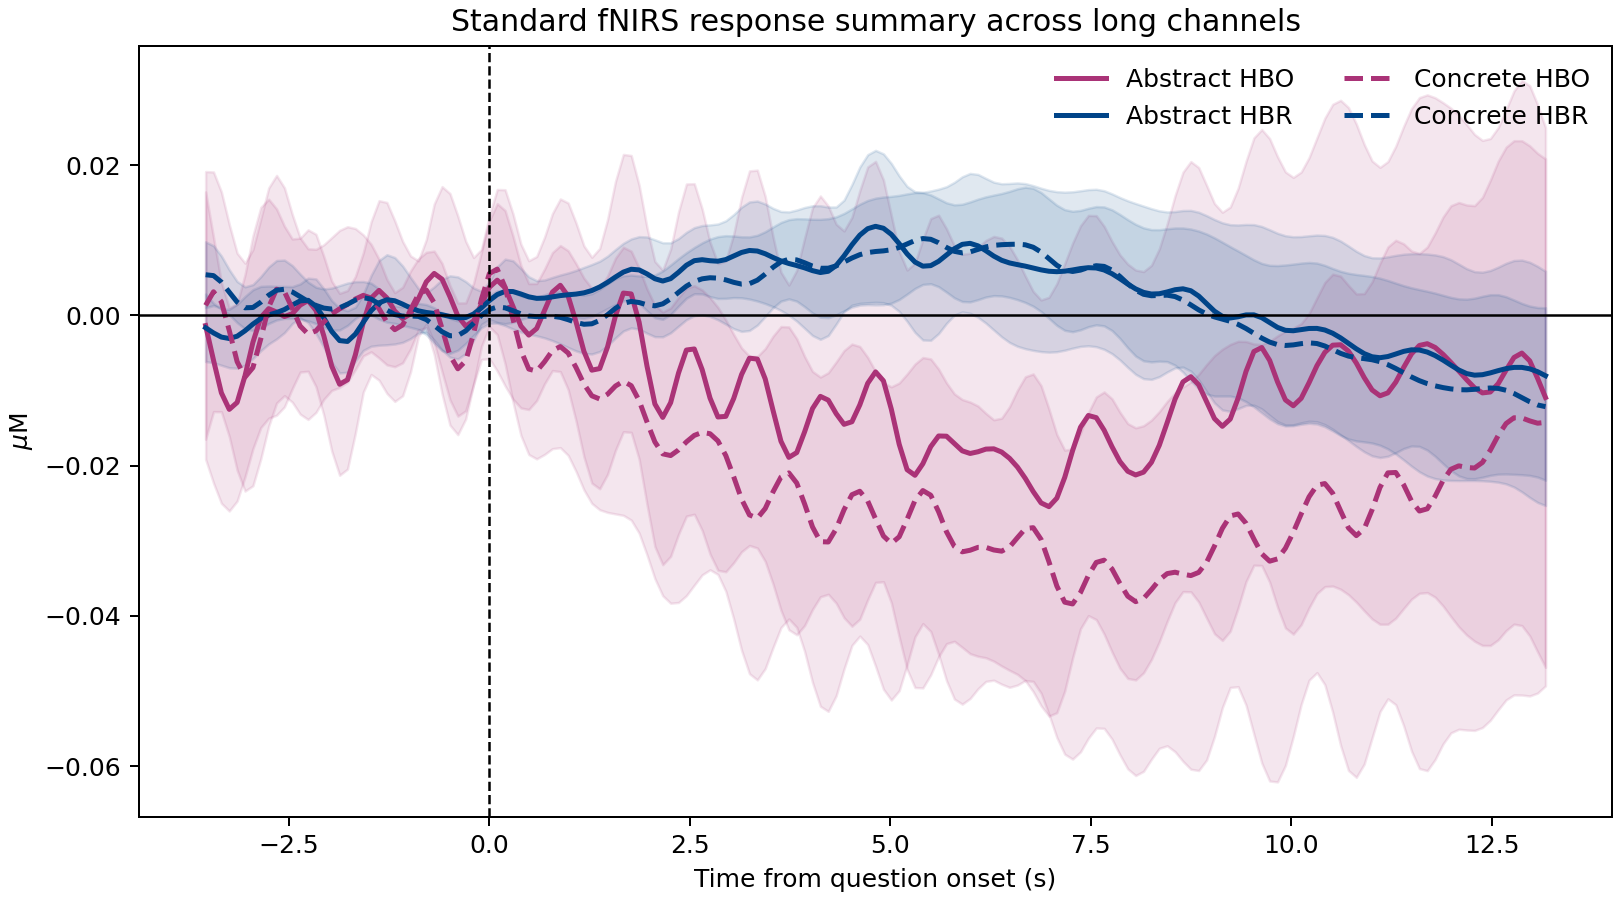
\includegraphics[width=0.92\linewidth]{../../figures/step7_visualization/standard_fnirs_compare.png}
\caption{Standard fNIRS waveform comparison across long channels for the Step~7 included trial set.}
\end{figure}
\begin{figure}[H]
\centering
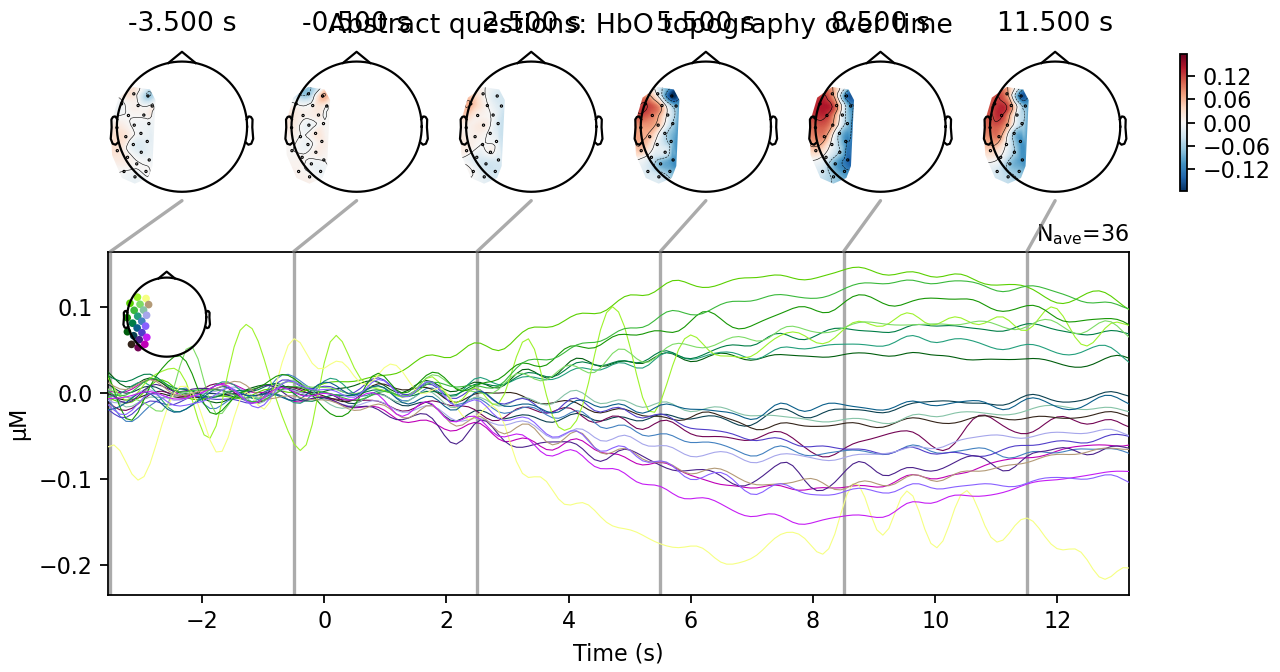
\includegraphics[width=0.95\linewidth]{../../figures/step7_visualization/abstract_hbo_joint.png}
\caption{Grand-average HbO topography over time for Abstract questions using the Step~7 included trial set.}
\end{figure}
\begin{figure}[H]
\centering
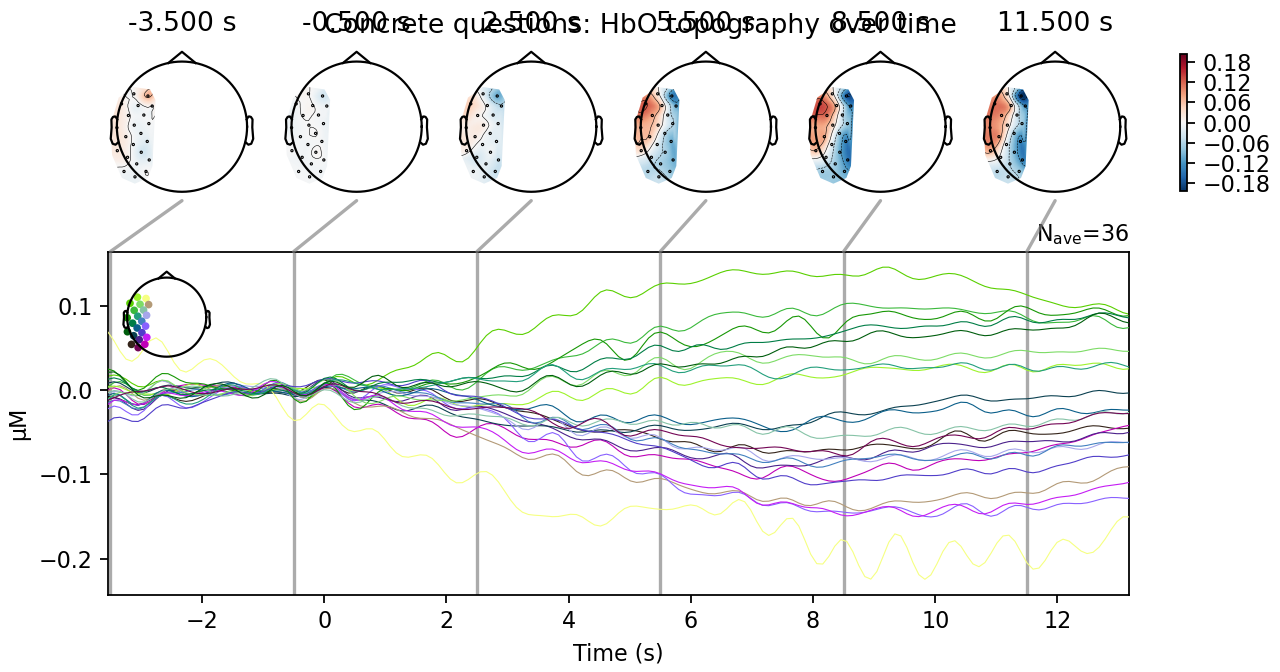
\includegraphics[width=0.95\linewidth]{../../figures/step7_visualization/concrete_hbo_joint.png}
\caption{Grand-average HbO topography over time for Concrete questions using the Step~7 included trial set.}
\end{figure}
\begin{figure}[H]
\centering
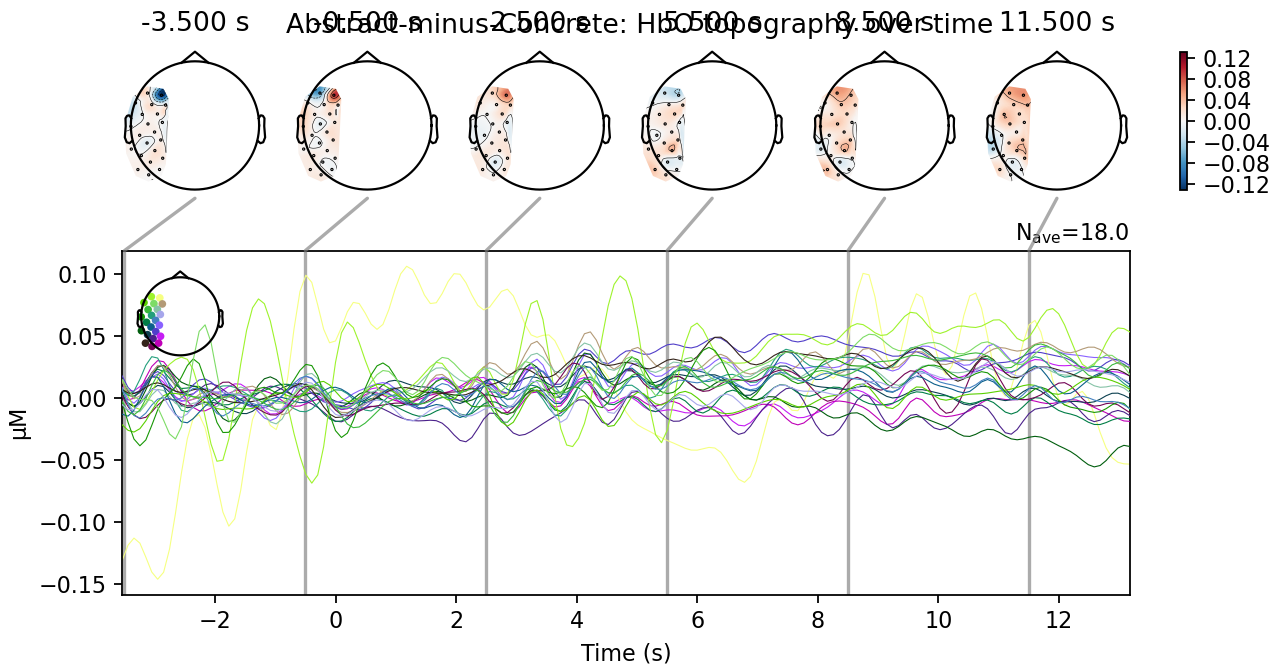
\includegraphics[width=0.95\linewidth]{../../figures/step7_visualization/abstract_minus_concrete_hbo_joint.png}
\caption{Grand-average Abstract-minus-Concrete HbO topography over time.}
\end{figure}
\begin{figure}[H]
\centering
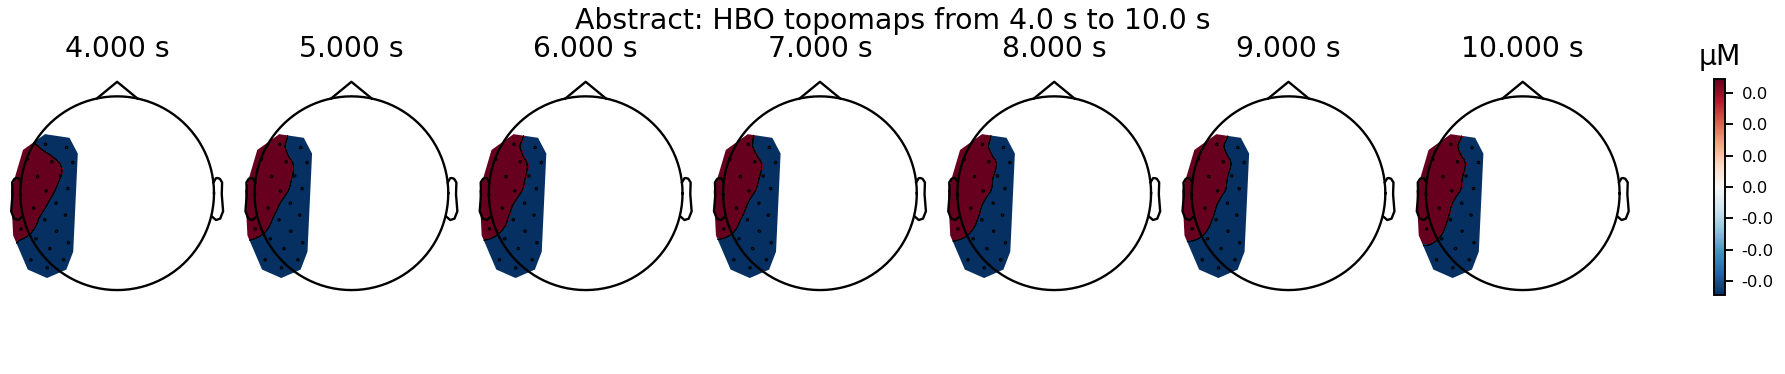
\includegraphics[width=0.48\linewidth]{../../figures/step7_visualization/abstract_hbo_topomap_series.png}
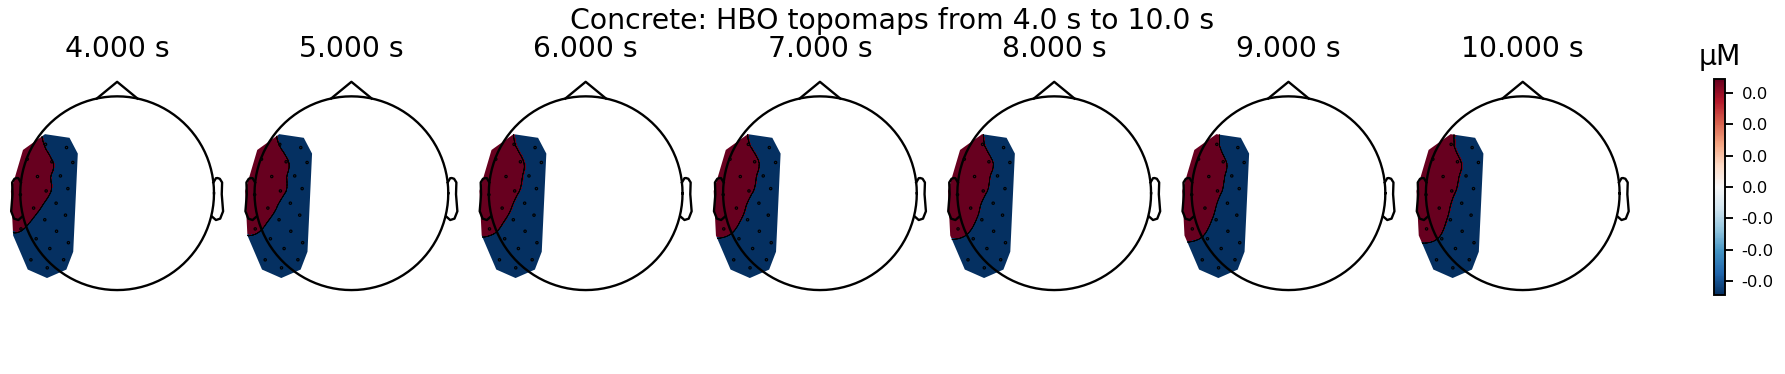
\includegraphics[width=0.48\linewidth]{../../figures/step7_visualization/concrete_hbo_topomap_series.png}
\caption{HbO topographic time series from 4.0~s to 10.0~s for the Abstract and Concrete conditions.}
\end{figure}
\begin{figure}[H]
\centering
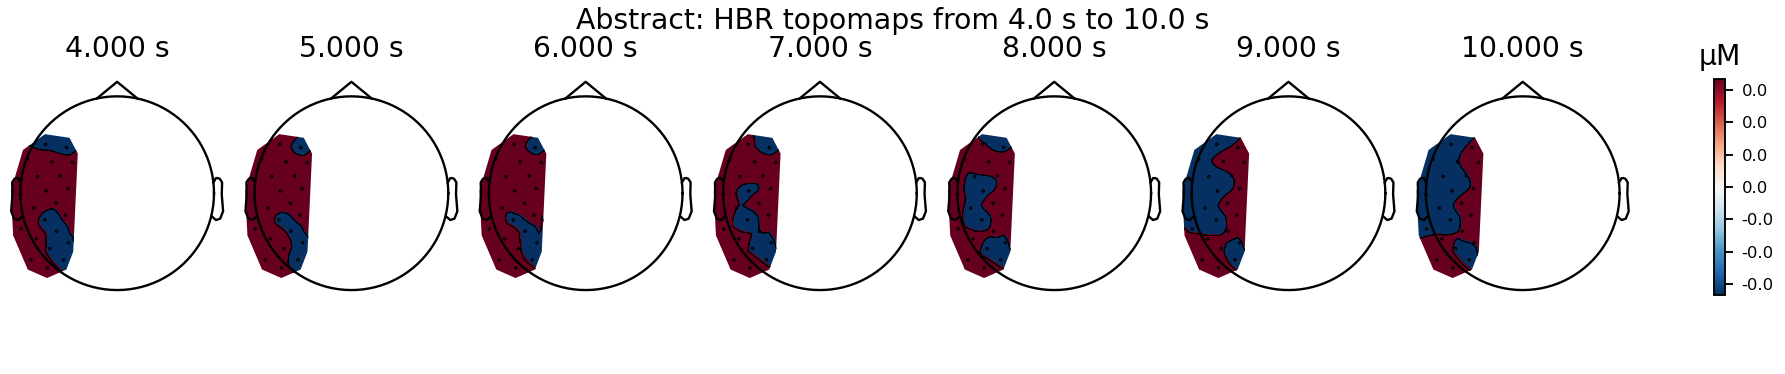
\includegraphics[width=0.48\linewidth]{../../figures/step7_visualization/abstract_hbr_topomap_series.png}
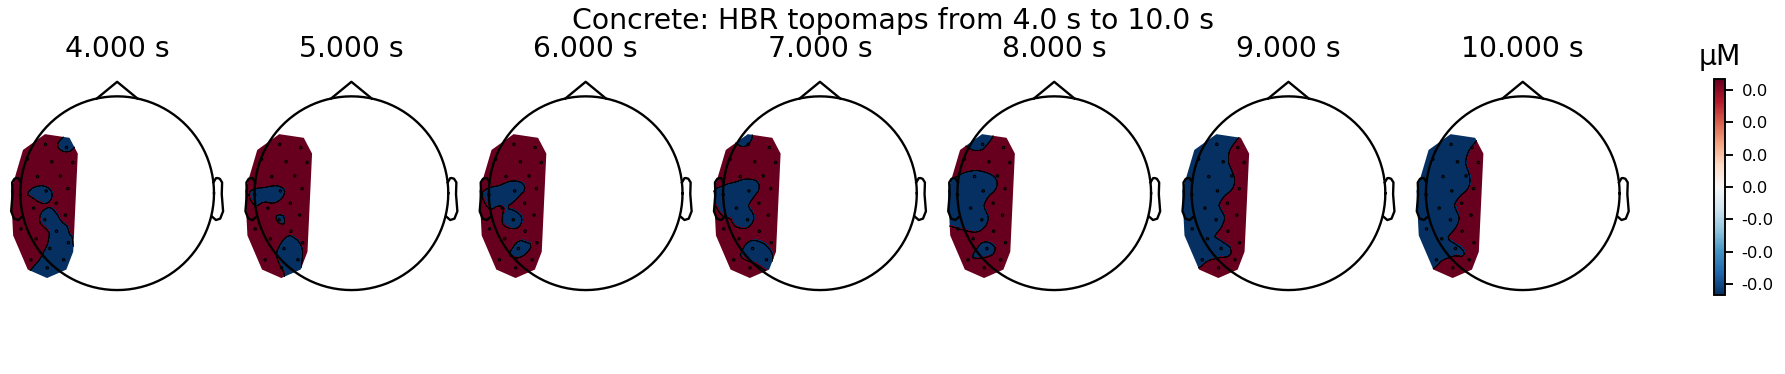
\includegraphics[width=0.48\linewidth]{../../figures/step7_visualization/concrete_hbr_topomap_series.png}
\caption{HbR topographic time series from 4.0~s to 10.0~s for the Abstract and Concrete conditions.}
\end{figure}
\begin{figure}[H]
\centering
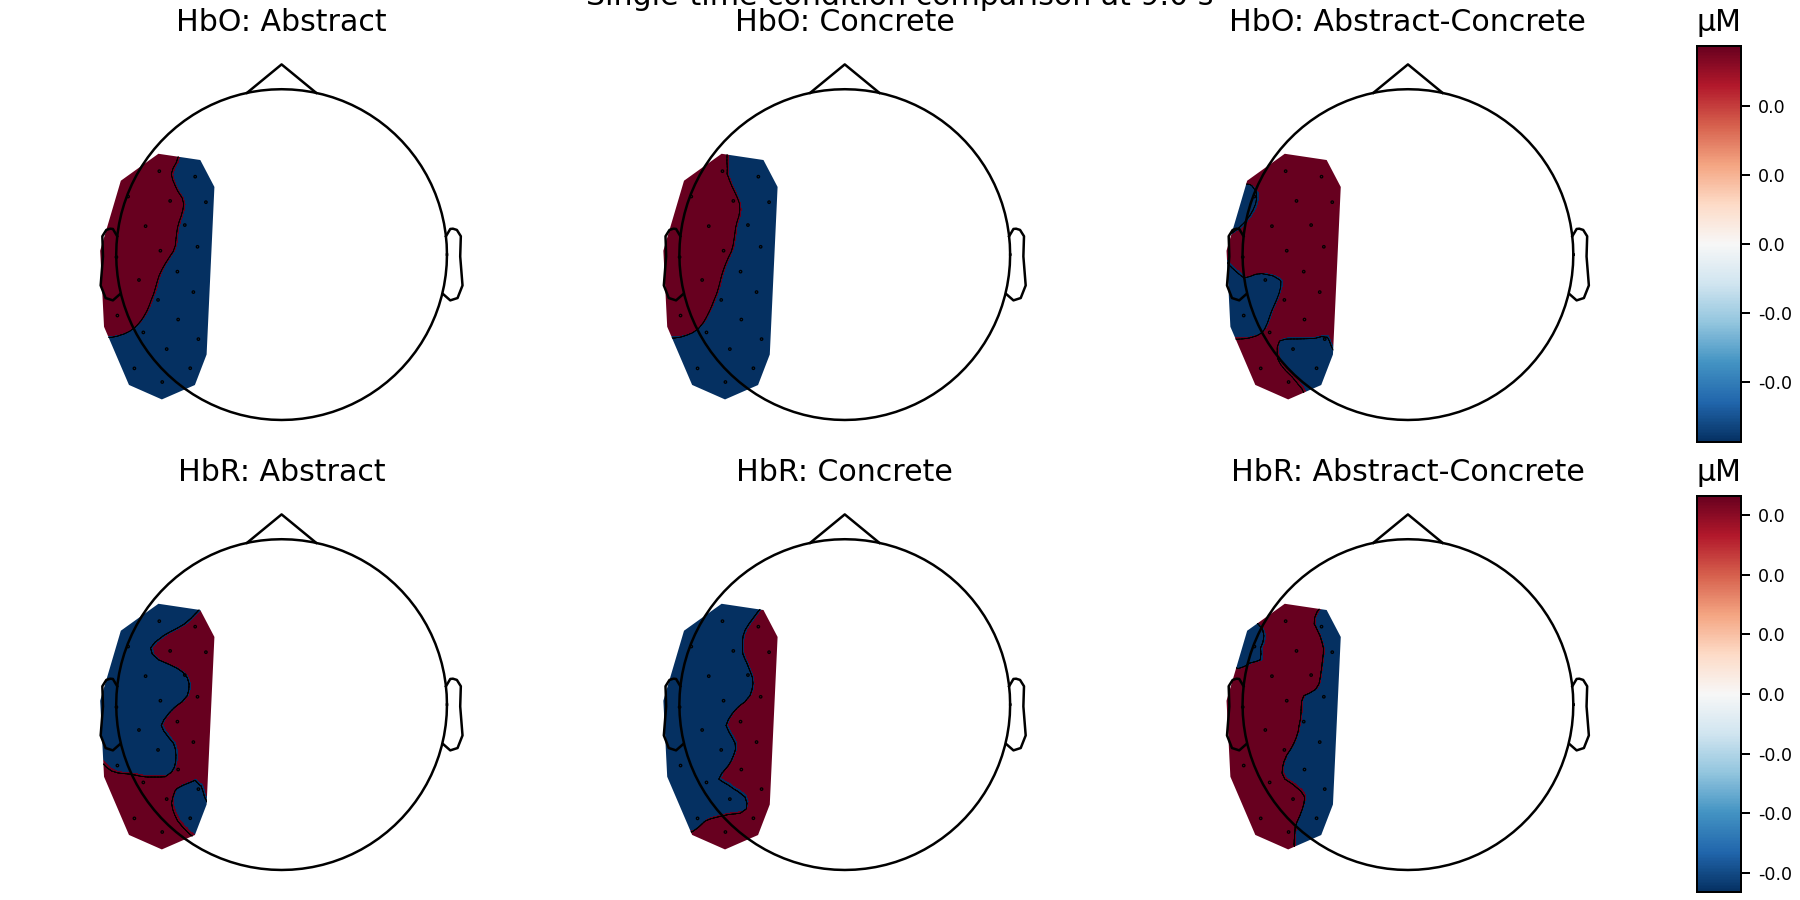
\includegraphics[width=0.95\linewidth]{../../figures/step7_visualization/abstract_concrete_single_time_comparison.png}
\caption{Single-time comparison at 9.0~s for Abstract, Concrete, and Abstract-minus-Concrete topographies for both HbO and HbR.}
\end{figure}
\begin{figure}[H]
\centering
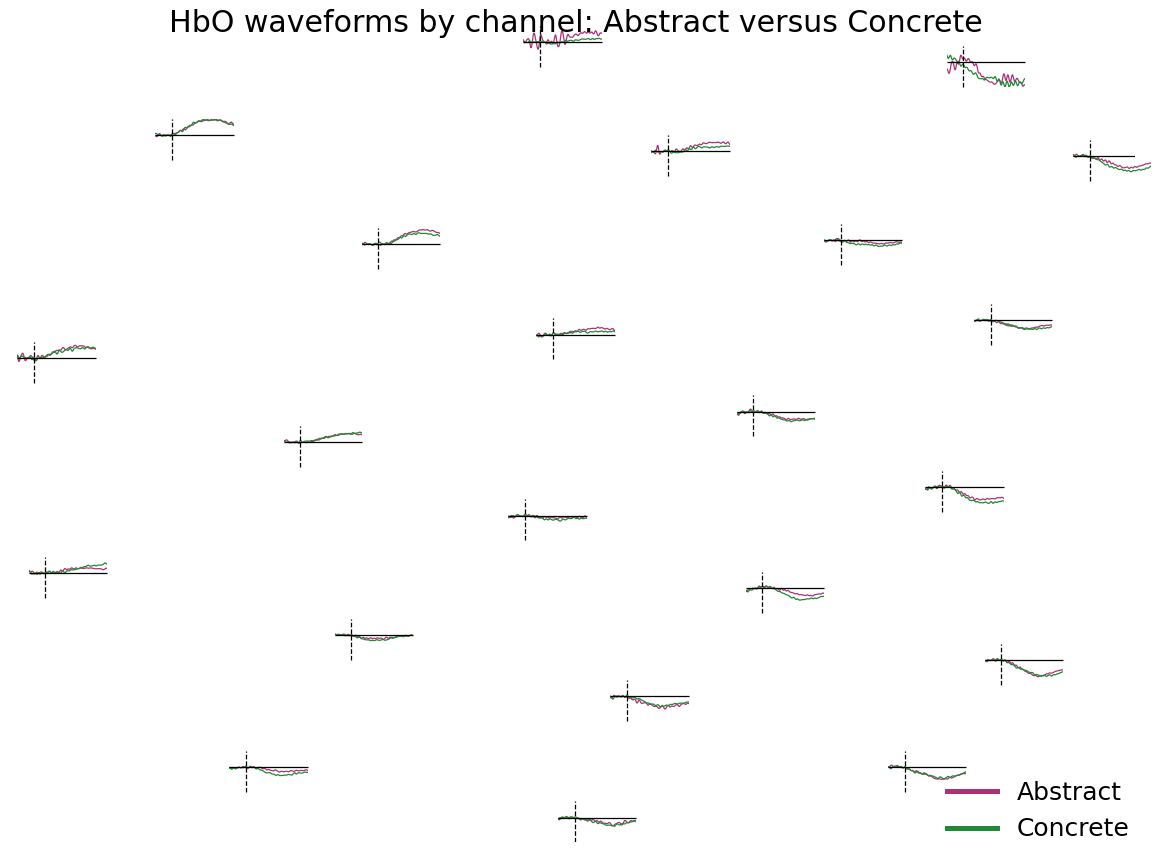
\includegraphics[width=0.95\linewidth]{../../figures/step7_visualization/abstract_concrete_hbo_evoked_topo.png}
\caption{HbO waveforms by long channel, overlaid for Abstract and Concrete, to show what drives the descriptive topographic differences.}
\end{figure}
\end{document}
